\documentclass[14pt,letterpaper]{article}
\usepackage[margin=2cm,includefoot]{geometry}
\usepackage[spanish]{babel}

\usepackage[%  
    colorlinks=true,
    pdfborder={0 0 0},
    linkcolor=blue
]{hyperref}

\usepackage{xcolor}
\usepackage{amsmath}
\usepackage{multicol}
\usepackage{graphicx}
\usepackage{qtree}
\usepackage{tikz}

\graphicspath{ {./img/} }

\title{Programa 01}
\author{Diego Méndez Medina}
\date{}


\begin{document}

\ttfamily
\maketitle
\rmfamily

\begin{itemize}
\item {\bf Alcanzabilidad}
  \begin{enumerate}
  \item Dar su forma canónica

    Al tener una grafica no dirigida $G=(V,A)$, decimos que dos
    vértices, $s$ y $t$, son {\it alcanzables} cuando existe
    un camino que no repite vértices de $s$ a $t$ en $G$.

    {\bf Enunciado de optimización:} Sea $G=(V,A)$ una gráfica simple no dirigida,
    y $s$ y $t$ dos vértices diferentes.  Determinar el camino
    de $s$ a $t$ con el mínimo número de aristas.

    {\bf Enunciado de decisión:} Sea $G=(V,A)$ una gráfica simple no dirigida,
    $s$ y $t$ dos vértices diferentes y $k$ un entero positivo. Nos preguntamos, ¿Existe
    un camino de $s$ a $t$ de a lo más $k$ vértices?.
    
  \item Diseñar un algoritmo no-determinístico polinomial.

    Asusimos la presencia de una gráfica aleatoria y el algoritmo
    no-determinista es el siguiente:

    \begin{enumerate}
    \item Seleccionamos dos vértices $s$ y $t$.
    \item Inicializamos un conjunto de aristas vacio, $M$.
    \item Iteramos sobre las aristas, y generamos
      un numero ``aleatorio'' $r$, si es par agregamos
      la arista a $M$ has juntar las $k$ aristas.
    \end{enumerate}
    
    Para verificar si la solución propuesta se debe hacer lo siguiente:

    \begin{enumerate}
    \item Lo primero es verificar que $s$ y $t$ figuren en alguna arista, en caso
      de ser correcto continuamos si no regresamos {\tt NO}.
    \item Para todas las aristas donde figure $s$ hay que seguir el camino
      que nos lleve dentro del conjunto solucion, en caso de que el camino
      se ``rompa'' en algúna arista regresamos {\tt NO}.
    \item Regresamos {\tt Sí}, si encontramos a $t$ antes de completar los $k$
      vértices.
    \end{enumerate}
  \item Implementación

    Para la implementación se utilizó C, se fijo $k=10$, 15 aristas y 11 vértices.

    Para compilar hacer cualquiera de las dos opciones:

    \begin{align*}
      \text{{\tt src/\$}}\ & \text{{\tt make compile\_alcance}}\\\\
      \text{{\tt src/\$}}\ & \text{{\tt gcc -o alcance alcance.c grafica.c}}\\\\      
    \end{align*}

    Para ejecutar:
    
    \begin{align*}
      \text{{\tt src/\$}}\ & \text{{\tt ./alcance}}\\\\
    \end{align*}

    \newpage
    Para compilar {\bf Y} ejecutar:
    
    \begin{align*}
      \text{{\tt src/\$}}\ & \text{{\tt make problema\_alcance}}\\\\
    \end{align*}

  \item Capturas de ejecución:

    \begin{figure}[h]
      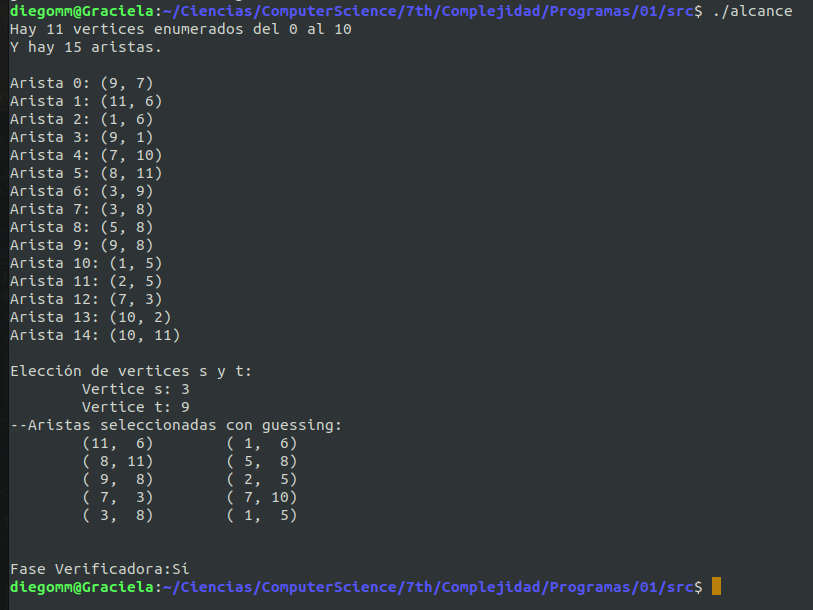
\includegraphics[width=10cm]{alcance_1.png}
      \centering
    \end{figure}

    \hfill\break
    
    \begin{figure}[h]
      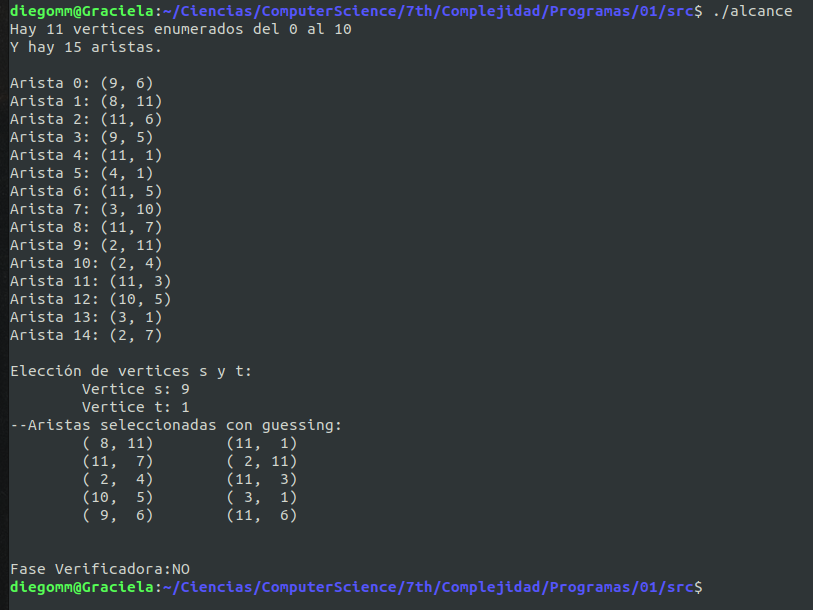
\includegraphics[width=10cm]{alcance_2.png}
      \centering
    \end{figure}

    \hfill\break
    
    \begin{figure}[h]
      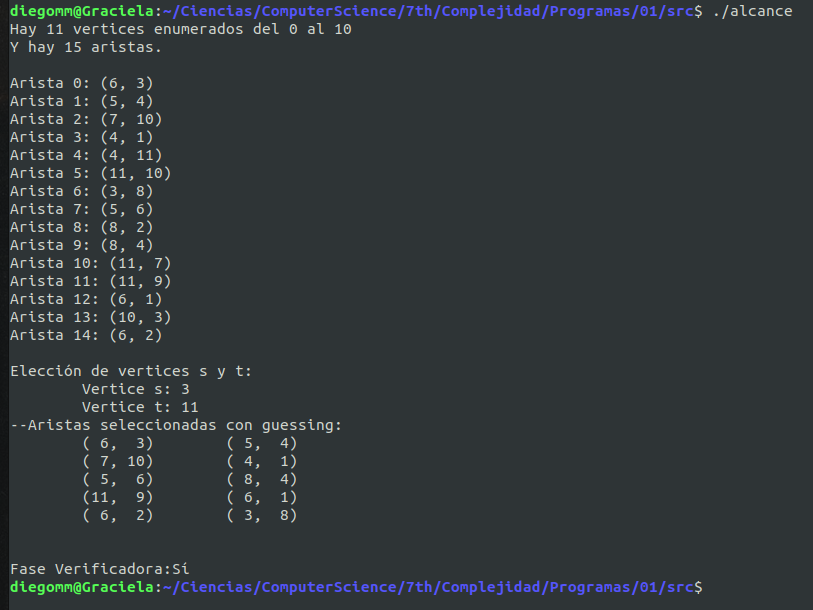
\includegraphics[width=10cm]{alcance_3.png}
      \centering
    \end{figure}

    \hfill\break
    
    \begin{figure}[h]
      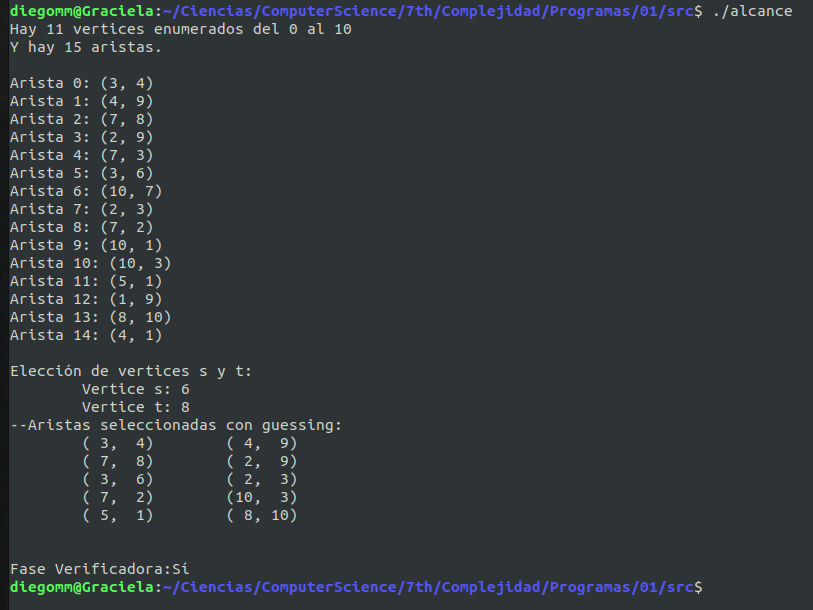
\includegraphics[width=10cm]{alcance_4.png}
      \centering
    \end{figure}

    \hfill\break
    
    \begin{figure}[h]
      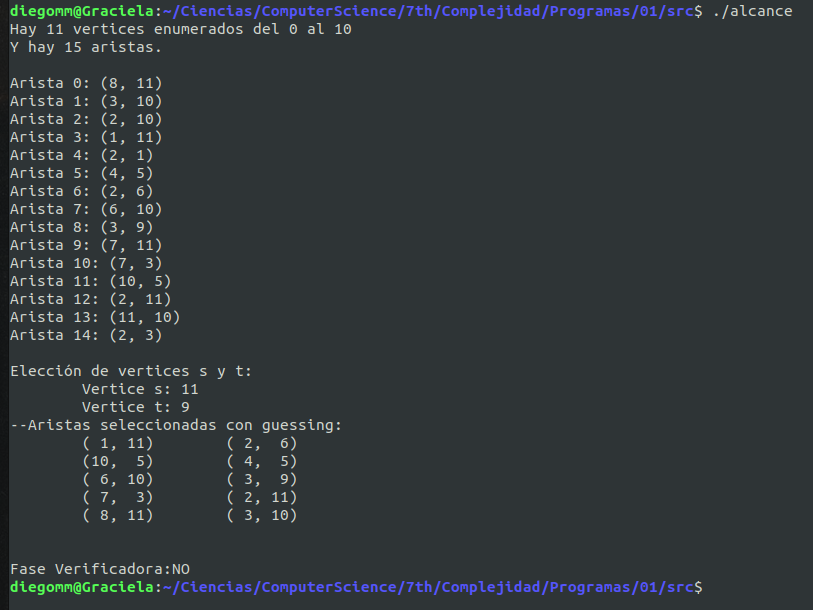
\includegraphics[width=10cm]{alcance_5.png}
      \centering
    \end{figure}

    \hfill\break
  \end{enumerate}

  \newpage
  
\item {\bf 3-SAT}
  \begin{enumerate}
  \item Dar su forma canónica

    Al tener una expresión lógica $\psi$ de primer orden en forma CNF, decimos que
    es {\it satisfasible} cuando existe una interpretación $I:VAR\rightarrow \{true,\,false\}$,
    tal que $\psi$ es verdadera.
    
  \item Diseñar un algoritmo no-determinístico polinomial.

    Suponemos ya existe la $\psi$ en forma CNF con 10 variables conocidas. El algoritmo
    no deterministico es el siguiente:
    \begin{enumerate}
    \item Creamos un conjunto de variables que funcionara como modelo.
    \item Iteramos sobre las diez variables, sacamos un número aleatorio, si
      es par a esa variable se le asigna el valor verdadero.
    \end{enumerate}

    Así ya tenemos el ejemplar propuesto, en tiempo lineal checamos la formula $psi$
    si alguna clausula falla regresamos {\tt NO}, si checamos todas las clausulas
    entonces regresamos {\tt Sí}.
    
  \item Implementación

    Para compilar hacer cualquiera de las dos opciones:

    \begin{align*}
      \text{{\tt src/\$}}\ & \text{{\tt make compile\_sat}}\\\\
      \text{{\tt src/\$}}\ & \text{{\tt gcc -o sat 3sat.c FOL.c}}\\\\      
    \end{align*}

    Para ejecutar:
    
    \begin{align*}
      \text{{\tt src/\$}}\ & \text{{\tt ./sat}}\\\\
    \end{align*}

    Para compilar {\bf Y} ejecutar:
    
    \begin{align*}
      \text{{\tt src/\$}}\ & \text{{\tt make problema\_3sat}}\\\\
    \end{align*}

  \item Capturas de ejecución:

    \begin{figure}[h]
      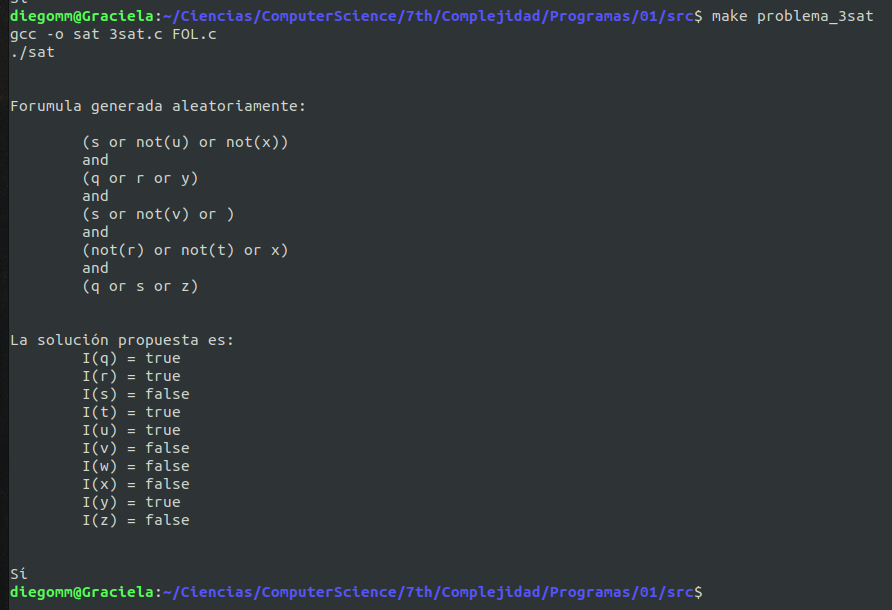
\includegraphics[width=10cm]{sat_1.png}
      \centering
    \end{figure}

    \hfill\break
    
    \begin{figure}[h]
      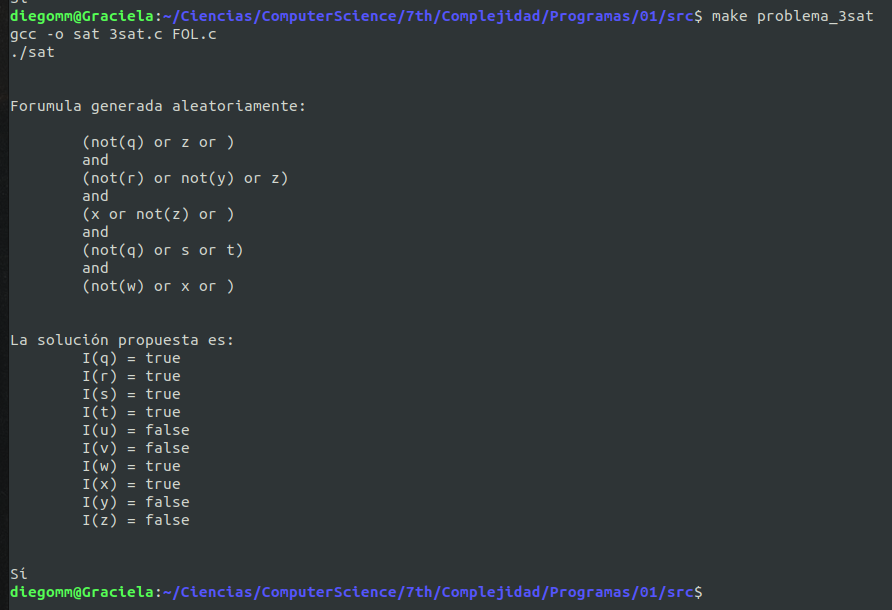
\includegraphics[width=10cm]{sat_2.png}
      \centering
    \end{figure}

    \hfill\break
    
    \begin{figure}[h]
      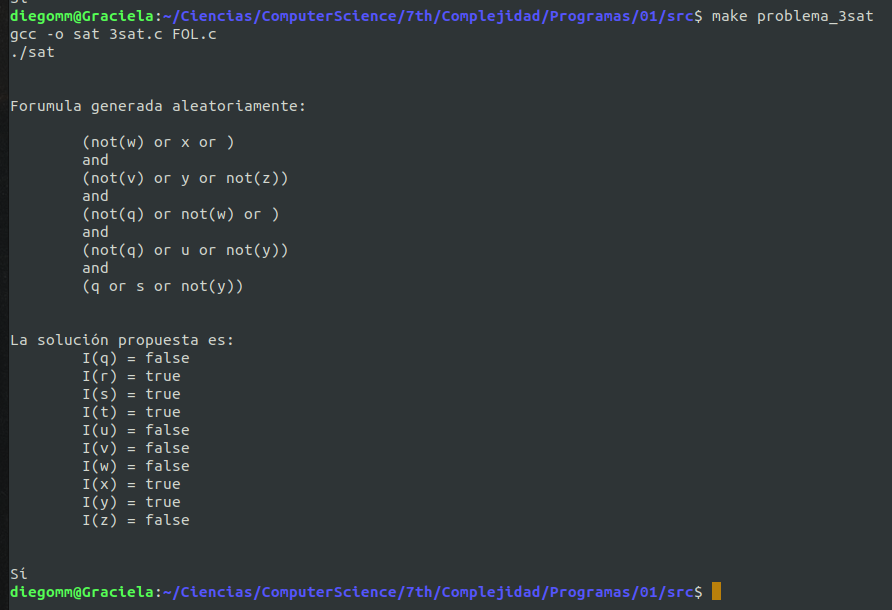
\includegraphics[width=10cm]{sat_3.png}
      \centering
    \end{figure}

    \hfill\break
    
    \begin{figure}[h]
      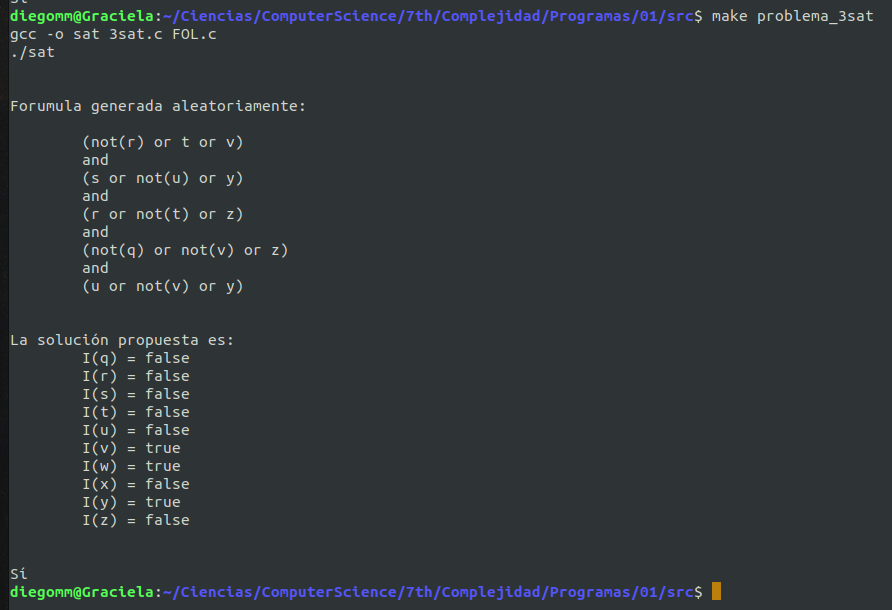
\includegraphics[width=10cm]{sat_4.png}
      \centering
    \end{figure}

    \hfill\break
    
    \begin{figure}[h]
      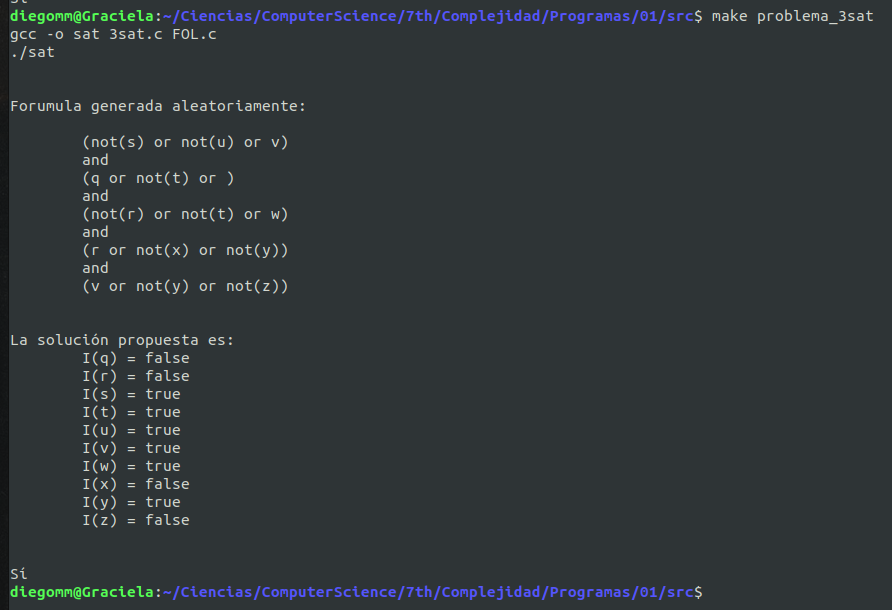
\includegraphics[width=10cm]{sat_5.png}
      \centering
    \end{figure}

    \hfill\break
    
  \end{enumerate}
\end{itemize}
\end{document}



